% =====================================================================
%  Modulo 3 -- Inferenza nelle reti bayesiane
%  Lezione 4 (Exact inference) e Lezione 5 (Approximate inference)
% =====================================================================

\chapter{Inferenza esatta}

\textit{Lezione 4.} Una rete bayesiana rappresenta in modo compatto una
distribuzione congiunta. Ora vediamo come \textbf{calcolare probabilità a
posteriori} direttamente dalle distribuzioni condizionate locali, senza mai
costruire la congiunta completa.

Esempio guida per tutto il capitolo: la rete dell'allarme.

\begin{center}
\begin{tikzpicture}[bn]
  \node[var] (B) {$B$};
  \node[var, right=22mm of B] (E) {$E$};
  \node[var, below right=8mm and 6mm of B] (A) {$A$};
  \node[obs, below left=8mm and 6mm of A] (J) {$J$};
  \node[obs, below right=8mm and 6mm of A] (M) {$M$};
  \draw[->] (B) -- (A); \draw[->] (E) -- (A);
  \draw[->] (A) -- (J); \draw[->] (A) -- (M);
\end{tikzpicture}
\qquad
\small
\begin{tabular}[b]{cc|c}
  $B$ & $E$ & $P(a\mid B,E)$ \\ \midrule
  T & T & 0.95 \\ T & F & 0.94 \\ F & T & 0.29 \\ F & F & 0.001
\end{tabular}\quad
\begin{tabular}[b]{c|cc}
  $A$ & $P(j\mid A)$ & $P(m\mid A)$ \\ \midrule
  T & 0.90 & 0.70 \\ F & 0.05 & 0.01
\end{tabular}
\end{center}
con $P(b)=0.001$, $P(e)=0.002$. In grigio le variabili osservate. La rete
fattorizza la congiunta come
\[
  \Pb(B,E,A,J,M) = \Pb(B)\,\Pb(E)\,\Pb(A\mid B,E)\,\Pb(J\mid A)\,\Pb(M\mid A).
\]
Notazione: $b$ indica $B=\mathit{true}$, $\neg b$ indica $B=\mathit{false}$, e
lo stesso per $e,a,j,m$.

% =====================================================================
\section{Tipi di inferenza}
% =====================================================================

John e Mary chiamano entrambi dicendo che l'allarme suona. Cosa ci può dire il
modello?
\begin{itemize}
  \item \textbf{Query marginale}: quanto è probabile un furto?
        $\Pb(\mathit{Burglary}\mid j, m)$.
  \item \textbf{Query congiunta}: quanto è probabile ogni combinazione di furto e
        terremoto? $\Pb(\mathit{Burglary},\mathit{Earthquake}\mid j, m)$.
  \item \textbf{Spiegazione}: quali eventi nascosti spiegano meglio le chiamate
        osservate? Le probabilità a posteriori permettono di confrontare le
        spiegazioni possibili.
\end{itemize}

Le stesse probabilità servono anche a prendere decisioni e ad analizzare il
modello:
\begin{itemize}
  \item \textbf{Decisioni ottime}: conviene mandare qualcuno a controllare la
        casa? Servono le probabilità degli eventi rilevanti più costi e
        benefici di ogni azione.
  \item \textbf{Valore dell'informazione}: conviene verificare se c'è stato un
        terremoto prima di decidere? Si valuta se un'evidenza in più ne
        giustifica il costo.
  \item \textbf{Analisi di sensitività}: quanto cambierebbe la conclusione se il
        tasso di falsi positivi dell'allarme fosse diverso?
\end{itemize}
Tutti questi compiti si basano sullo stesso calcolo: rispondere a una
\emph{query probabilistica}.

\dfn{Query probabilistica (su una rete bayesiana)}{
  Una \textbf{query probabilistica} chiede la distribuzione condizionata delle
  variabili di query $\mathbf{Y}$ data l'evidenza osservata $\mathbf{E}=\mathbf{e}$:
  \[
    \Pb(\mathbf{Y}\mid\mathbf{E}=\mathbf{e}).
  \]
  \begin{itemize}
    \item \textbf{query marginale}: una sola variabile, $\Pb(X_i\mid\mathbf{E}=\mathbf{e})$;
    \item \textbf{query congiunta}: più variabili, $\Pb(X_i,X_j\mid\mathbf{E}=\mathbf{e})$.
  \end{itemize}
  Le restanti variabili sono \textbf{nascoste} (hidden).
}

\textbf{Domanda chiave:} come si calcolano queste distribuzioni direttamente dai
modelli locali della rete?

% =====================================================================
\section{Inferenza per enumerazione}
% =====================================================================

\subsection{La query}

Vogliamo $\Pb(B\mid j,m)$:
\begin{itemize}
  \item variabile di query: $B$;
  \item evidenza: $J=\mathit{true}$, $M=\mathit{true}$;
  \item variabili nascoste: $E$, $A$.
\end{itemize}
Servono entrambi i valori di $B$: $P(b\mid j,m)$ e $P(\neg b\mid j,m)$.

\subsection{Da una posteriori a due probabilità congiunte}

Per definizione di probabilità condizionata
\[
  P(b\mid j,m) = \frac{P(b,j,m)}{P(j,m)},
  \qquad
  P(j,m) = P(b,j,m) + P(\neg b,j,m).
\]
Il denominatore è lo stesso per entrambi i valori di $B$. Basta quindi saper
calcolare $P(b,j,m)$ e $P(\neg b,j,m)$ dalla rete, e poi normalizzare.

\subsection{Enumerare le possibilità nascoste}

Fissiamo $B=\mathit{true}$ insieme all'evidenza $j,m$. Non sappiamo se ci sia
stato un terremoto né se l'allarme abbia suonato: ci sono quattro assegnamenti
di $(E,A)$, mutuamente esclusivi, e li sommiamo:
\[
  P(b,j,m) = P(b,e,a,j,m) + P(b,e,\neg a,j,m) + P(b,\neg e,a,j,m) + P(b,\neg e,\neg a,j,m).
\]
Poi si ripete con $B=\mathit{false}$.

\subsection{Leggere le probabilità dalle CPT}

Per ogni assegnamento completo si sceglie \emph{una} entrata da ciascuna
distribuzione locale e si moltiplicano, grazie alla fattorizzazione della rete.

\ex{Un assegnamento completo}{
  Mondo $B=E=A=J=M=\mathit{true}$:
  \begin{center}
  \begin{tabular}{lll}
    \toprule
    Nodo & Entrata della CPT & Valore \\ \midrule
    $B$ & $P(b)$ & 0.001 \\
    $E$ & $P(e)$ & 0.002 \\
    $A$ & $P(a\mid b,e)$ & 0.95 \\
    $J$ & $P(j\mid a)$ & 0.90 \\
    $M$ & $P(m\mid a)$ & 0.70 \\ \bottomrule
  \end{tabular}
  \end{center}
  \[
    P(b,e,a,j,m) = 0.001\cdot0.002\cdot0.95\cdot0.90\cdot0.70 = 0.000001197.
  \]
}

Tenendo fissi $B=\mathit{true}$ e l'evidenza, si calcola il prodotto per ognuno
dei quattro assegnamenti di $(E,A)$:
\begin{center}
\begin{tabular}{cc|l}
  $E$ & $A$ & Prodotto delle entrate scelte \\ \midrule
  T & T & $P(b)P(e)P(a\mid b,e)P(j\mid a)P(m\mid a)$ \\
  T & F & $P(b)P(e)P(\neg a\mid b,e)P(j\mid \neg a)P(m\mid \neg a)$ \\
  F & T & $P(b)P(\neg e)P(a\mid b,\neg e)P(j\mid a)P(m\mid a)$ \\
  F & F & $P(b)P(\neg e)P(\neg a\mid b,\neg e)P(j\mid \neg a)P(m\mid \neg a)$
\end{tabular}
\end{center}
La loro somma è il \textbf{peso non normalizzato} $q_b = P(b,j,m)$. Con altri
quattro prodotti si ottiene $q_{\neg b} = P(\neg b,j,m)$.

\subsection{La procedura}

\dfn{Inferenza per enumerazione}{
  Si risponde a una query sommando su tutti gli assegnamenti delle variabili
  nascoste. Ogni probabilità congiunta si calcola come prodotto delle entrate
  delle CPT locali:
  \[
    \Pb(X\mid\mathbf{e}) = \alpha\,\Pb(X,\mathbf{e})
    = \alpha\sum_{\mathbf{h}}\prod_{i=1}^{n} P(x_i\mid \mathit{parents}(X_i)).
  \]
  Per la nostra query:
  \begin{enumerate}
    \item fissa l'evidenza $j,m$;
    \item per ogni valore di $B$, enumera gli assegnamenti di $E,A$;
    \item moltiplica le entrate delle CPT e somma, ottenendo $q_b$ e $q_{\neg b}$;
    \item normalizza:
      \[
        \Pb(B\mid j,m) = \alpha\langle q_b, q_{\neg b}\rangle,
        \qquad \alpha = \frac{1}{q_b+q_{\neg b}}.
      \]
  \end{enumerate}
}

\nt{
  \textbf{Cosa abbiamo guadagnato?} Le somme si calcolano direttamente dalle CPT,
  senza memorizzare la tabella della congiunta completa. Rispetto
  all'enumerazione sulla congiunta (capitolo precedente) lo spazio scende da
  $O(d^n)$ a $O(n)$. Il tempo invece resta esponenziale.
}

\subsection{Albero di valutazione e calcoli ripetuti}

Il calcolo di $P(b,j,m)$ si può riorganizzare spostando ogni fattore il più a
sinistra possibile:
\[
  P(b,j,m) = P(b)\sum_{e}P(e)\sum_{a}P(a\mid b,e)\,P(j\mid a)\,P(m\mid a).
\]
L'enumerazione ricorsiva in profondità valuta questa espressione visitando un
albero:

\begin{center}
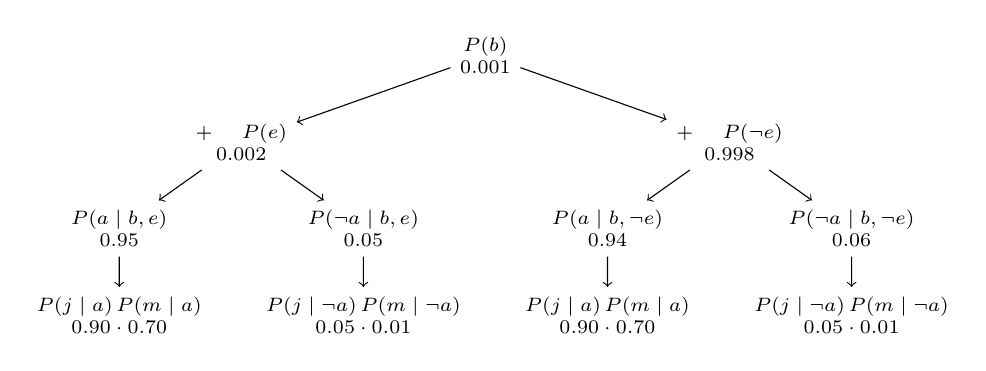
\begin{tikzpicture}[
    level distance=11mm,
    every node/.style={font=\scriptsize, align=center},
    level 1/.style={sibling distance=62mm},
    level 2/.style={sibling distance=31mm},
    level 3/.style={sibling distance=31mm},
    edge from parent/.style={draw, ->}]
  \node {$P(b)$\\0.001}
    child {node {$+$ \quad $P(e)$\\0.002}
      child {node {$P(a\mid b,e)$\\0.95}
        child {node {$P(j\mid a)\,P(m\mid a)$\\$0.90\cdot0.70$}}}
      child {node {$P(\neg a\mid b,e)$\\0.05}
        child {node {$P(j\mid\neg a)\,P(m\mid\neg a)$\\$0.05\cdot0.01$}}}}
    child {node {$+$ \quad $P(\neg e)$\\0.998}
      child {node {$P(a\mid b,\neg e)$\\0.94}
        child {node {$P(j\mid a)\,P(m\mid a)$\\$0.90\cdot0.70$}}}
      child {node {$P(\neg a\mid b,\neg e)$\\0.06}
        child {node {$P(j\mid\neg a)\,P(m\mid\neg a)$\\$0.05\cdot0.01$}}}};
\end{tikzpicture}
\end{center}

\mprop{Complessità dell'enumerazione su una rete}{
  Con $n$ variabili di dominio al più $d$, l'enumerazione ricorsiva in
  profondità richiede
  \begin{itemize}
    \item spazio $O(n)$: non costruisce mai la congiunta;
    \item tempo $O(d^n)$: visita tutti gli assegnamenti delle nascoste.
  \end{itemize}
}

\nt{
  \textbf{È inefficiente:} gli stessi prodotti, come $P(j\mid a)P(m\mid a)$, sono
  ricalcolati in più rami dell'albero.\\
  \textbf{Si può fare meglio?} Sì: calcolando una volta sola le espressioni
  ripetute, memorizzandole e riutilizzandole. È l'idea dell'eliminazione di
  variabili.
}

\subsection{L'algoritmo}

\begin{algorithm}[H]
\SetKwFunction{EA}{Enumeration-Ask}
\SetKwFunction{EAll}{Enumerate-All}
\SetKwProg{Fn}{function}{}{}
\Fn{\EA{$X$, $\mathbf{e}$, $bn$} \KwRet{una distribuzione su $X$}}{
  \KwIn{$X$ variabile di query; $\mathbf{e}$ valori osservati per le variabili
        $\mathbf{E}$; $bn$ rete con variabili $\mathit{Vars}[bn]=\{X\}\cup\mathbf{E}\cup\mathbf{Y}$}
  $\mathbf{Q}(X) \leftarrow$ distribuzione su $X$, inizialmente vuota\;
  \ForEach{valore $x_i$ di $X$}{
    estendi $\mathbf{e}$ con $X = x_i$\;
    $\mathbf{Q}(x_i) \leftarrow$ \EAll{$\mathit{Vars}[bn]$, $\mathbf{e}$}\;
  }
  \KwRet{$\mathrm{Normalize}(\mathbf{Q}(X))$}\;
}
\BlankLine
\Fn{\EAll{$vars$, $\mathbf{e}$} \KwRet{un numero reale}}{
  \lIf{$vars$ è vuota}{\KwRet{1.0}}
  $Y \leftarrow \mathrm{First}(vars)$\;
  \eIf{$Y$ ha valore $y$ in $\mathbf{e}$}{
    \KwRet{$P(y\mid \mathit{Parents}(Y)) \times$ \EAll{$\mathrm{Rest}(vars)$, $\mathbf{e}$}}\;
  }{
    \KwRet{$\sum_y P(y\mid \mathit{Parents}(Y)) \times$ \EAll{$\mathrm{Rest}(vars)$, $\mathbf{e}\cup\{Y=y\}$}}\;
  }
}
\caption{Inferenza per enumerazione}
\end{algorithm}

Le variabili in $\mathit{Vars}[bn]$ vanno elencate in ordine topologico, così
quando si arriva a $Y$ i valori dei suoi genitori sono già fissati.

% =====================================================================
\section{Eliminazione di variabili}
% =====================================================================

Vogliamo sempre $\Pb(B\mid j,m)$. Il prodotto $P(j\mid a)P(m\mid a)$ dipende solo
da $A$: lo si può calcolare una volta per ogni valore di $A$, memorizzarlo e
riusarlo per tutti i valori di $B$ ed $E$.

\dfn{Eliminazione di variabili (variable elimination)}{
  Algoritmo di inferenza \textbf{esatta} che somma via (\emph{sums out}) le
  variabili nascoste una alla volta, memorizzando i risultati intermedi come
  \textbf{fattori} per non ripetere calcoli.
}

\subsection{Fattori}

\dfn{Fattore}{
  Un \textbf{fattore} è una funzione non negativa di un insieme di variabili.
  Per variabili discrete è una tabella con un valore per ogni assegnamento.
  Il suo \textbf{scope} è l'insieme delle variabili da cui dipende.
}

\ex{Un fattore ottenuto fissando l'evidenza}{
  La CPT $\Pb(J\mid A)$ coinvolge $J$ e $A$. Osservando $J=\mathit{true}$ si
  tengono solo le righe con $J=\mathit{true}$ e si ottiene un fattore su $A$:
  \begin{center}
  \begin{tabular}{cc|c}
    $A$ & $J$ & $P(J\mid A)$ \\ \midrule
    T & T & \textbf{0.90} \\ T & F & 0.10 \\ F & T & \textbf{0.05} \\ F & F & 0.95
  \end{tabular}
  \quad$\xrightarrow{\;J=\mathit{true}\;}$\quad
  \begin{tabular}{c|c}
    $A$ & $f_J(A)=P(j\mid A)$ \\ \midrule T & 0.90 \\ F & 0.05
  \end{tabular}
  \end{center}
  Un fattore \emph{non} deve sommare a 1: qui $0.90+0.05=0.95$.
}

\subsection{Passo 1: fattori iniziali e restrizione all'evidenza}

Ogni nodo ha un modello locale, che è una tabella di valori non negativi: è
quindi un fattore. Il prodotto dei cinque fattori è la congiunta. Fissando
l'evidenza $J=\mathit{true}$, $M=\mathit{true}$ si ottengono i fattori iniziali:
\begin{center}
\begin{tabular}{lll}
  \toprule
  Nodo & Modello locale & Fattore iniziale \\ \midrule
  $B$ & $\Pb(B)$ & $f_B(B)=\Pb(B)$ \\
  $E$ & $\Pb(E)$ & $f_E(E)=\Pb(E)$ \\
  $A$ & $\Pb(A\mid B,E)$ & $f_A(A,B,E)=\Pb(A\mid B,E)$ \\
  $J$ & $\Pb(J\mid A)$ & $f_J(A)=\Pb(J=\mathit{true}\mid A)$ \\
  $M$ & $\Pb(M\mid A)$ & $f_M(A)=\Pb(M=\mathit{true}\mid A)$ \\ \bottomrule
\end{tabular}
\end{center}
Solo i modelli di $J$ e $M$ sono ristretti dall'evidenza: $J,M$ sono fissati,
mentre $A$ resta variabile. $f_M(A)$ vale 0.70 per $A=\mathit{true}$ e 0.01 per
$A=\mathit{false}$.

\subsection{Passo 2: scrivere il calcolo con i fattori}

Per ogni valore $b'\in\{\mathit{true},\mathit{false}\}$ della query si calcola il
peso non normalizzato $q(b')=P(B=b',j,m)$, sommando sulle nascoste $E,A$:
\[
  q(b') = \sum_E\sum_A f_B(b')\,f_E(E)\,f_A(A,b',E)\,f_J(A)\,f_M(A).
\]
I fattori che non dipendono da una variabile sommata si portano fuori dalla
sua somma:
\[
  q(b') = f_B(b')\sum_E f_E(E)\left[\sum_A f_A(A,b',E)\,f_J(A)\,f_M(A)\right].
\]
Si valuta prima la somma interna su $A$, poi quella su $E$, infine si normalizza:
$P(B=b'\mid j,m) = \alpha\,q(b')$.

Servono due sole operazioni sui fattori.

\dfn{Operazione 1: prodotto puntuale (pointwise product)}{
  Il prodotto di due fattori moltiplica le entrate che \textbf{concordano sui
  valori delle variabili condivise}. Il risultato ha come scope l'\textbf{unione}
  degli scope:
  \[
    (f\times g)(\mathbf{X},\mathbf{Y},\mathbf{Z}) = f(\mathbf{X},\mathbf{Y})\cdot g(\mathbf{Y},\mathbf{Z}).
  \]
  Ad esempio un fattore su $A,B$ per uno su $B,E$ dà un fattore su $A,B,E$.
}

\ex{$g(A) = f_J(A)\,f_M(A)$}{
  \begin{center}
  \begin{tabular}{c|ccc}
    $A$ & $f_J(A)$ & $f_M(A)$ & $g(A)$ \\ \midrule
    T & 0.90 & 0.70 & 0.63 \\
    F & 0.05 & 0.01 & 0.0005
  \end{tabular}
  \end{center}
  Questi due prodotti si riusano per ogni assegnamento di $B,E$.
}

\dfn{Operazione 2: sommare via una variabile (summing out)}{
  Per eliminare una variabile $Z$ da un fattore, per ogni assegnamento delle
  variabili rimanenti si somma sui valori di $Z$:
  \[
    h(\mathbf{X}) = \sum_{z} f(\mathbf{X}, Z=z).
  \]
  Il nuovo fattore non dipende più da $Z$: ogni sua entrata include tutti i
  valori di $Z$.
}

\ex{Sommare via $A$}{
  I fattori che coinvolgono $A$ sono $f_A(A,B,E)=\Pb(A\mid B,E)$ e $g(A)$. Per
  ogni coppia $(B,E)$ si moltiplicano le entrate corrispondenti per
  $A=\mathit{true}$ e $A=\mathit{false}$ e si sommano. Per $B=E=\mathit{true}$:
  \begin{center}
  \begin{tabular}{c|ccc}
    $A$ & $P(A\mid b,e)$ & $g(A)$ & Prodotto \\ \midrule
    T & 0.95 & 0.63 & 0.5985 \\
    F & 0.05 & 0.0005 & 0.000025
  \end{tabular}
  \end{center}
  \[
    P(j,m\mid b,e) = 0.5985 + 0.000025 = 0.598525.
  \]
  Ripetendo per ogni coppia si ottiene
  $h(B,E)=\sum_A f_A(A,B,E)\,g(A) = P(a\mid B,E)\cdot0.63 + P(\neg a\mid B,E)\cdot0.0005$:
  \begin{center}
  \begin{tabular}{cc|lc}
    $B$ & $E$ & Calcolo & $h(B,E)$ \\ \midrule
    T & T & $0.95\cdot0.63 + 0.05\cdot0.0005$ & 0.598525 \\
    T & F & $0.94\cdot0.63 + 0.06\cdot0.0005$ & 0.592230 \\
    F & T & $0.29\cdot0.63 + 0.71\cdot0.0005$ & 0.183055 \\
    F & F & $0.001\cdot0.63 + 0.999\cdot0.0005$ & 0.0011295
  \end{tabular}
  \end{center}
}

\subsection{Passo 3: sommare via $E$}

Eliminata $A$, la query diventa
$\Pb(B\mid j,m) = \alpha\, f_B(B)\sum_E f_E(E)\,h(B,E)$. Definiamo
$k(B)=\sum_E f_E(E)\,h(B,E)$; con $P(e)=0.002$ e $P(\neg e)=0.998$:
\begin{align*}
  k(\mathit{true})  &= 0.002\cdot0.598525 + 0.998\cdot0.592230 = 0.59224259,\\
  k(\mathit{false}) &= 0.002\cdot0.183055 + 0.998\cdot0.0011295 = 0.001493351.
\end{align*}
Ora restano solo fattori sulla variabile di query: $\Pb(B\mid j,m)=\alpha\,f_B(B)\,k(B)$.

\subsection{Passo 4: moltiplicare i fattori rimasti e normalizzare}

\begin{align*}
  q_b      &= 0.001\cdot0.59224259 = 0.00059224259,\\
  q_{\neg b} &= 0.999\cdot0.001493351 = 0.001491857649,
\end{align*}
\[
  \Pb(B\mid j,m) = \frac{\langle q_b, q_{\neg b}\rangle}{q_b+q_{\neg b}}
  \approx \langle 0.2842,\ 0.7158\rangle.
\]

\nt{
  \textbf{Interpretazione.} Se John e Mary chiamano entrambi, la probabilità a
  posteriori di un furto è circa il \textbf{28.4\%}.\\
  Enumerazione ed eliminazione di variabili danno lo \emph{stesso} risultato:
  l'eliminazione riorganizza soltanto il calcolo per riusare i risultati
  intermedi.
}

\subsection{La procedura generale}

\mprop{Eliminazione di variabili}{
  \begin{enumerate}
    \item \textbf{Fissa l'evidenza}: restringi le distribuzioni locali ai valori
          osservati, ottenendo i fattori iniziali.
    \item \textbf{Scegli un ordine} di eliminazione per le variabili nascoste.
    \item Per ogni variabile nascosta $Z$:
      \begin{itemize}
        \item raccogli tutti i fattori correnti che coinvolgono $Z$;
        \item moltiplicali e somma via $Z$;
        \item sostituisci i fattori raccolti con il fattore risultante.
      \end{itemize}
    \item \textbf{Moltiplica} i fattori rimasti.
    \item \textbf{Normalizza} per ottenere la posteriori sulle variabili di query.
  \end{enumerate}
  Una variabile si elimina solo dopo aver combinato \emph{tutti} i fattori che
  al momento dipendono da essa. I fattori che non la contengono restano
  invariati.
}

\begin{algorithm}[H]
\SetKwFunction{ElA}{Elimination-Ask}
\SetKwProg{Fn}{function}{}{}
\Fn{\ElA{$X$, $\mathbf{e}$, $bn$} \KwRet{una distribuzione su $X$}}{
  \KwIn{$X$ variabile di query; $\mathbf{e}$ evidenza; $bn$ rete che specifica
        $\Pb(X_1,\dots,X_n)$}
  $\mathit{factors} \leftarrow [\,]$\;
  \ForEach{$\mathit{var}$ in $\mathrm{Order}(\mathit{Vars}[bn])$}{
    $\mathit{factors} \leftarrow [\mathrm{Make\text{-}Factor}(\mathit{var},\mathbf{e}) \mid \mathit{factors}]$\;
    \If{$\mathit{var}$ è una variabile nascosta}{
      $\mathit{factors} \leftarrow \mathrm{Sum\text{-}Out}(\mathit{var},\mathit{factors})$\;
    }
  }
  \KwRet{$\mathrm{Normalize}(\mathrm{Pointwise\text{-}Product}(\mathit{factors}))$}\;
}
\caption{Eliminazione di variabili}
\end{algorithm}

\nt{
  \textbf{Ordine di eliminazione.} \emph{Qualunque} ordine dà un algoritmo
  corretto, ma il costo cambia molto. Euristica: scegliere ogni volta la
  variabile che minimizza la dimensione del prossimo fattore da costruire.
}

% =====================================================================
\section{Rendere l'eliminazione più efficiente}
% =====================================================================

\subsection{Variabili irrilevanti: le foglie non osservate}

Consideriamo una nuova query sulla rete dell'allarme:
$\Pb(\mathit{JohnCalls}\mid\mathit{Burglary}=\mathit{true}) = \Pb(J\mid b)$.
Qui la query è $J$, l'evidenza è $B=\mathit{true}$ e le nascoste sono $E,A,M$.
La chiamata di Mary non è né chiesta né osservata: la sua CPT serve davvero?

\[
  \Pb(J\mid b) = \alpha\sum_e P(e)\sum_a P(a\mid b,e)\,\Pb(J\mid a)
  \underbrace{\sum_m P(m\mid a)}_{=1}.
\]
Per ogni valore di $A$, $\sum_m P(m\mid A) = P(M=\mathit{true}\mid A)+P(M=\mathit{false}\mid A)=1$. Quindi
\[
  \Pb(J\mid b) = \alpha\sum_e P(e)\sum_a P(a\mid b,e)\,\Pb(J\mid a):
\]
$M$ e la sua CPT si possono omettere e il risultato è identico.

\nt{
  \textbf{Perché funziona?} $M$ è una \textbf{foglia non osservata}: non ha figli
  e nessun altro fattore la contiene, quindi la sua somma vale 1. Se invece
  $M$ fosse osservata, si selezionerebbe $P(m\mid A)$ invece di sommare, e quel
  fattore in generale cambierebbe il risultato.
}

\subsection{Regola grafica: il sottografo ancestrale}

\thm{Sottografo ancestrale}{
  Per una query $\Pb(X\mid\mathbf{E}=\mathbf{e})$ basta conservare
  \begin{itemize}
    \item la variabile di query $X$;
    \item le variabili di evidenza $\mathbf{E}$;
    \item tutti gli \textbf{antenati} di $X$ e di $\mathbf{E}$.
  \end{itemize}
  Tutti gli altri nodi si possono rimuovere prima dell'inferenza.
}
\pf{Idea}{
  Si rimuovono ripetutamente le foglie non osservate e non interrogate: ognuna
  contribuisce una somma pari a 1, come $M$ sopra. Rimossa una foglia, i suoi
  genitori possono diventare foglie a loro volta. Il processo si ferma
  esattamente al sottografo ancestrale di $\{X\}\cup\mathbf{E}$.
}

Per $\Pb(J\mid b)$ i nodi conservati sono $\{J,B,A,E\}$: $\mathit{MaryCalls}$ ne è
fuori e si rimuove.

\subsection{Variabili irrilevanti per d-separazione}

\ex{Rete dello studente: $\Pb(\mathit{Job}\mid \mathit{Grade}=g, \mathit{SAT}=s)$}{
  \begin{center}
  \begin{tikzpicture}[bn, node distance=8mm and 10mm]
    \node[blk] (D) {$\mathit{Difficulty}$};
    \node[blk, right=28mm of D] (I) {$\mathit{Intelligence}$};
    \node[obs, below right=8mm and -4mm of D] (G) {$\mathit{Grade}$};
    \node[obs, below right=8mm and 2mm of I] (S) {$\mathit{SAT}$};
    \node[var, below=of G] (L) {$\mathit{Letter}$};
    \node[var, below right=8mm and 14mm of L] (J) {$\mathit{Job}$};
    \node[var, below left=8mm and 4mm of L, dashed] (H) {$\mathit{Happy}$};
    \draw[->] (D) -- (G); \draw[->] (I) -- (G); \draw[->] (I) -- (S);
    \draw[->] (G) -- (L); \draw[->] (L) -- (J); \draw[->] (S) -- (J);
    \draw[->, dashed] (G) to[bend right=30] (H); \draw[->, dashed] (J) -- (H);
  \end{tikzpicture}
  \end{center}
  In grigio l'evidenza, in rosso i nodi resi irrilevanti dalla d-separazione,
  tratteggiato il nodo rimosso con il sottografo ancestrale.
  \begin{enumerate}
    \item \textbf{Sottografo ancestrale.} $\mathit{Happy}$ non è né query né
          evidenza, né antenato di una di esse: si rimuove.
    \item \textbf{D-separazione.} $\mathit{Difficulty}$ e $\mathit{Intelligence}$
          sono antenati, ma servono le loro distribuzioni? Guardiamo i trail
          verso $\mathit{Job}$:
      \begin{itemize}
        \item $\mathit{Difficulty}\to\mathit{Grade}\to\mathit{Letter}\to\mathit{Job}$:
              $\mathit{Grade}$ è un non-collider osservato, quindi è bloccato;
        \item $\mathit{Intelligence}\to\mathit{Grade}\to\mathit{Letter}\to\mathit{Job}$:
              bloccato da $\mathit{Grade}$;
        \item $\mathit{Intelligence}\to\mathit{SAT}\to\mathit{Job}$:
              bloccato da $\mathit{SAT}$, anch'esso non-collider osservato.
      \end{itemize}
      Quindi
      $\cind{\mathit{Job}}{\{\mathit{Difficulty},\mathit{Intelligence}\}}{\mathit{Grade},\mathit{SAT}}$.
  \end{enumerate}
}

\thm{Irrilevanza per d-separazione}{
  Se $Y$ è d-separata dalla variabile di query $X$ dalle variabili di evidenza
  $\mathbf{E}$, allora $Y$ è irrilevante come evidenza aggiuntiva per la query:
  \[
    \Pb(X\mid\mathbf{E}=\mathbf{e}, Y=y) = \Pb(X\mid\mathbf{E}=\mathbf{e}),
  \]
  ogni volta che l'evento condizionante ha probabilità positiva.
}

Nell'esempio dello studente il calcolo si riduce a una sola variabile
nascosta, $\mathit{Letter}$:
\[
  \Pb(\mathit{Job}\mid g,s) = \sum_{l}\Pb(\mathit{Job}\mid \mathit{Letter}=l,\mathit{SAT}=s)\,P(\mathit{Letter}=l\mid\mathit{Grade}=g).
\]
Servono solo i modelli locali di $\mathit{Letter}$ e $\mathit{Job}$.

\nt{La semplificazione dipende dalla \emph{specifica} query e dalla sua evidenza.}

% =====================================================================
\section{Complessità dell'eliminazione di variabili}
% =====================================================================

\subsection{Dimensione dei fattori e ordine di eliminazione}

Gran parte del costo dell'eliminazione sta nel memorizzare i fattori
intermedi. Con variabili booleane un fattore su 2 variabili ha $2^2=4$ entrate,
su 10 variabili $2^{10}=1024$, su 20 variabili $2^{20}$.

\mprop{Costo dell'eliminazione di variabili}{
  Un limite standard per il tempo (e lo spazio) è
  \[
    O(n\,d^{k}),
  \]
  dove $n$ è il numero di variabili, $d$ il massimo numero di valori per
  variabile e $k$ lo scope più grande di un prodotto di fattori formato prima di
  sommare via una variabile.
}

\nt{
  \textbf{L'ordine conta.} Ordini diversi creano fattori intermedi di dimensioni
  diverse, cioè cambiano $k$. Fattori più piccoli richiedono meno tempo e meno
  memoria.
}

\subsection{Effetto della struttura della rete}

\dfn{Polytree}{
  Una rete bayesiana è un \textbf{polytree} (singly connected) se due nodi
  qualsiasi sono collegati da \textbf{al più un cammino} quando si ignora la
  direzione degli archi.
}

\mprop{Polytree}{
  Su un polytree, con un ordine di eliminazione adatto, i fattori intermedi
  restano piccoli rispetto ai modelli locali. Con domini e numero di genitori
  limitati, l'inferenza esatta richiede tempo \textbf{lineare} nel numero di
  nodi.
}

\thm{Inferenza esatta in generale}{
  L'inferenza probabilistica esatta su reti bayesiane arbitrarie è
  \textbf{NP-hard}.
}

\nt{
  \textbf{Conseguenza pratica.} Una rete compatta non garantisce un'inferenza
  economica. Quando i fattori intermedi diventano troppo grandi, serve
  l'\emph{inferenza approssimata} (capitolo successivo).
}

\subsection{Altri approcci esatti: algoritmi di clustering}

\begin{itemize}
  \item L'eliminazione di variabili va bene per rispondere a \emph{singole} query.
        Calcolare le posteriori di tutte le $n$ variabili di un polytree costa
        però $O(n^2)$, perché si ripete una query per variabile.
  \item Gli \textbf{algoritmi di clustering} (\emph{join tree}) lo fanno in
        $O(n)$ e sono usati nei sistemi commerciali.
  \item Idea: unire nodi singoli in \textbf{meganodi} (cluster) fino a ottenere un
        polytree.
  \item Nel caso peggiore servono comunque CPT esponenzialmente grandi:
        l'alternativa sono i metodi approssimati.
\end{itemize}

% =====================================================================
\section{Esercizio d'esame: negozio online}
% =====================================================================

\qs{Testo}{
  Stai progettando un sistema di e-commerce che mostra annunci (\emph{ads}) di tre
  tipi: libri, giocattoli e vacanze. Il sito ne mostra uno alla volta, quindi
  il sistema deve indovinare quale tipo ha più probabilità di essere cliccato.
  Non hai profili verificati dei clienti, ma puoi stimare alcune
  caratteristiche dalla conoscenza del dominio e dai clic osservati:
  \begin{itemize}
    \item profilo: \textit{Young} ($y,\neg y$), \textit{Married} ($m,\neg m$),
          \textit{Wealthy} ($w,\neg w$), \textit{Children} ($c,\neg c$);
    \item comportamento di clic: \textit{Holiday} ($h,\neg h$), \textit{Book}
          ($b,\neg b$), \textit{Toy} ($t,\neg t$).
  \end{itemize}
  Come modelleresti il dominio con una rete bayesiana?
}

Si assume la rete seguente (abbreviazioni $Y,M,W,C,H,B,T$):

\begin{center}
\begin{tikzpicture}[bn, node distance=9mm and 8mm]
  \node[var] (Y) {$\mathit{Young}$};
  \node[var, right=30mm of Y] (M) {$\mathit{Married}$};
  \node[var, below=of Y] (W) {$\mathit{Wealthy}$};
  \node[var, below=of M] (C) {$\mathit{Children}$};
  \node[var, below left=9mm and 0mm of W] (H) {$\mathit{Holiday}$};
  \node[var, below right=9mm and 4mm of W] (B) {$\mathit{Book}$};
  \node[var, below right=9mm and 0mm of C] (T) {$\mathit{Toy}$};
  \draw[->] (Y) -- (W); \draw[->] (Y) -- (C); \draw[->] (M) -- (C);
  \draw[->] (W) -- (H); \draw[->] (W) -- (B); \draw[->] (C) -- (B);
  \draw[->] (C) -- (T);
\end{tikzpicture}
\end{center}
\[
  \Pb(Y,M,W,C,H,B,T) = \Pb(Y)\Pb(M)\Pb(W\mid Y)\Pb(C\mid Y,M)\,\Pb(H\mid W)\Pb(B\mid W,C)\Pb(T\mid C).
\]

\subsection*{Q1 -- Dedurre il profilo dai clic}

\qs{Q1}{
  Mostri una sequenza di annunci, registri quali vengono cliccati e usi questi
  dati per dedurre alcune caratteristiche del cliente. Quale pattern di
  ragionamento stai seguendo? Scrivi una query che usi come evidenza il
  comportamento di clic osservato.
}
\textbf{Risposta: ragionamento evidenziale (diagnostico).} Si ragiona dal
comportamento osservato (effetti) verso le variabili di profilo che lo spiegano
(cause). Ad esempio, se il cliente clicca un annuncio di vacanze ma non uno di
giocattoli:
\[
  \Pb(W, C\mid H=\mathit{true}, T=\mathit{false}),
\]
cioè una posteriori congiunta su ricchezza e genitorialità, con una
probabilità per ciascuna delle quattro combinazioni di $(W,C)$.

\subsection*{Q2 -- Contare i parametri liberi}

\qs{Q2}{Quanti valori indipendenti servono per definire completamente la rete?}
Tutte le variabili sono booleane: ogni configurazione dei genitori richiede
\emph{un} parametro libero, perché la probabilità di \textit{false} è il
complemento. Una variabile con $k$ genitori booleani ha quindi $2^k$
parametri.
\begin{center}
\begin{tabular}{lc}
  \toprule
  Distribuzione locale & Parametri liberi \\ \midrule
  $\Pb(Y)$ & 1 \\ $\Pb(M)$ & 1 \\ $\Pb(W\mid Y)$ & 2 \\ $\Pb(C\mid Y,M)$ & 4 \\
  $\Pb(H\mid W)$ & 2 \\ $\Pb(B\mid W,C)$ & 4 \\ $\Pb(T\mid C)$ & 2 \\ \midrule
  \textbf{Totale} & \textbf{16} \\ \bottomrule
\end{tabular}
\end{center}
Per confronto, la congiunta completa su 7 variabili booleane richiederebbe
$2^7-1=127$ parametri.

\subsection*{Q3 -- Una CPD per \textit{Children}}

\qs{Q3}{Definisci una CPD per \textit{Children}.}
I genitori di \textit{Children} sono \textit{Young} e \textit{Married}: per
ognuna delle quattro combinazioni va specificata $P(C=\mathit{true}\mid Y,M)$.
Una CPT possibile (quella usata nei calcoli successivi):
\begin{center}
\begin{tabular}{cc|cc}
  $Y$ & $M$ & $P(C=\mathit{true}\mid Y,M)$ & $P(C=\mathit{false}\mid Y,M)$ \\ \midrule
  T & T & 0.10 & 0.90 \\
  T & F & 0.01 & 0.99 \\
  F & T & 0.50 & 0.50 \\
  F & F & 0.45 & 0.55
\end{tabular}
\end{center}
Ad esempio $P(C=\mathit{true}\mid Y=\mathit{false},M=\mathit{true})=0.50$: in questo
modello un cliente non giovane e sposato ha figli con probabilità 0.50.

\nt{I valori numerici sono \emph{input} del modello: il grafo da solo non li
determina.}

\subsection*{Q4 -- $P(c\mid h)$ con eliminazione di variabili}

\qs{Q4}{
  Con i parametri
  $P(y)=0.4$, $P(m)=0.3$, $P(w\mid y)=0.05$, $P(w\mid\neg y)=0.2$,
  $P(h\mid w)=0.2$, $P(h\mid\neg w)=0.05$ e la CPT di Q3, calcola $P(c\mid h)$ con
  l'eliminazione di variabili.
}

\textbf{1. Query, evidenza, variabili rilevanti.} La query è $C$, l'evidenza
$H=\mathit{true}$ e le nascoste rilevanti sono $Y,M,W$. \textit{Book} e
\textit{Toy} sono foglie non osservate fuori dal sottografo ancestrale di
$\{C,H\}$: le loro CPT sommano a 1 e si omettono.

\textbf{2. Il calcolo prima di eliminare.} Per ogni valore $c'$ di $C$:
\[
  q(c') = P(C=c',h) = \sum_Y\sum_M\sum_W P(Y)P(M)P(W\mid Y)\,P(C=c'\mid Y,M)\,P(h\mid W).
\]
Ordine di eliminazione: $W, M, Y$. La variabile $C$ si tiene fino alla fine
perché è la query; l'evidenza $H=\mathit{true}$ è già fissata.

\textbf{3. Eliminare $W$.} I fattori che coinvolgono $W$ sono $\Pb(W\mid Y)$ e
$P(h\mid W)$:
\[
  \ell(Y) = \sum_W P(W\mid Y)\,P(h\mid W).
\]
\begin{center}
\begin{tabular}{c|lc}
  $Y$ & Calcolo & $\ell(Y)$ \\ \midrule
  T & $0.05\cdot0.20 + 0.95\cdot0.05$ & 0.0575 \\
  F & $0.20\cdot0.20 + 0.80\cdot0.05$ & 0.0800
\end{tabular}
\end{center}
Interpretazione: $\ell(Y)=P(h\mid Y)$, la probabilità di un clic sulle vacanze
per ciascuna fascia d'età, tenendo conto di entrambi i valori della ricchezza.

\textbf{4. Eliminare $M$.} I fattori che coinvolgono $M$ sono $\Pb(M)$ e
$\Pb(C\mid Y,M)$:
\[
  r(C,Y) = \sum_M P(M)\,P(C\mid Y,M).
\]
\begin{align*}
  r(\mathit{true},\mathit{true})  &= 0.30\cdot0.10 + 0.70\cdot0.01 = 0.037,\\
  r(\mathit{true},\mathit{false}) &= 0.30\cdot0.50 + 0.70\cdot0.45 = 0.465.
\end{align*}
\begin{center}
\begin{tabular}{c|cc}
  $Y$ & $r(C=\mathit{true},Y)$ & $r(C=\mathit{false},Y)$ \\ \midrule
  T & 0.037 & 0.963 \\ F & 0.465 & 0.535
\end{tabular}
\end{center}
In questo modello $r(C,Y)=\Pb(C\mid Y)$, quindi i valori per $C=\mathit{false}$
sono i complementi.

\textbf{5. Eliminare $Y$.} Restano $\Pb(Y)$, $\ell(Y)$ e $r(C,Y)$:
\[
  q(C) = \sum_Y P(Y)\,\ell(Y)\,r(C,Y).
\]
\begin{align*}
  q(\mathit{true})  &= 0.40\cdot0.0575\cdot0.037 + 0.60\cdot0.0800\cdot0.465
                     = 0.000851 + 0.022320 = 0.023171,\\
  q(\mathit{false}) &= 0.40\cdot0.0575\cdot0.963 + 0.60\cdot0.0800\cdot0.535 = 0.047829.
\end{align*}

\textbf{6. Normalizzare.} I due pesi sono probabilità congiunte:
$q(\mathit{true})=P(c,h)$ e $q(\mathit{false})=P(\neg c,h)$, con
$P(h)=0.023171+0.047829=0.071$. Quindi
\[
  P(c\mid h) = \frac{0.023171}{0.071}\approx 0.3264,
  \qquad
  \Pb(C\mid h)\approx\langle 0.3264,\ 0.6736\rangle.
\]
\textbf{Risposta:} dopo un clic su un annuncio di vacanze, la probabilità che
il cliente abbia figli è circa il \textbf{32.64\%}.

\subsection*{Q5 -- Estendere la rete con lo skateboard}

\qs{Q5}{
  Allarghi il business agli skateboard, molto popolari tra i \emph{giovani
  maschi}. Come estenderesti la rete per includere gli annunci di skateboard?
}
Si introducono $G=\mathit{Male}$ e $S=\mathit{Skateboard}$. La popolarità tra i
giovani maschi motiva la struttura $\mathit{Young}\to\mathit{Skateboard}\leftarrow\mathit{Male}$:

\begin{center}
\begin{tikzpicture}[bn, node distance=9mm and 8mm]
  \node[var] (Y) {$\mathit{Young}$};
  \node[var, left=18mm of Y] (G) {$\mathit{Male}$};
  \node[var, right=30mm of Y] (M) {$\mathit{Married}$};
  \node[var, below=of Y] (W) {$\mathit{Wealthy}$};
  \node[var, below=of M] (C) {$\mathit{Children}$};
  \node[var, below left=9mm and 18mm of W] (S) {$\mathit{Skateboard}$};
  \node[var, below left=9mm and 0mm of W] (H) {$\mathit{Holiday}$};
  \node[var, below right=9mm and 4mm of W] (B) {$\mathit{Book}$};
  \node[var, below right=9mm and 0mm of C] (T) {$\mathit{Toy}$};
  \draw[->] (Y) -- (W); \draw[->] (Y) -- (C); \draw[->] (M) -- (C);
  \draw[->] (W) -- (H); \draw[->] (W) -- (B); \draw[->] (C) -- (B);
  \draw[->] (C) -- (T);
  \draw[->] (G) -- (S); \draw[->] (Y) -- (S);
\end{tikzpicture}
\end{center}
L'estensione richiede $\Pb(G)$ e $\Pb(S\mid Y,G)$, cioè $1+4=5$ parametri liberi
in più con CPT booleane generiche.

\nt{Mettere \textit{Male} come radice separata è un'ulteriore \emph{assunzione
di indipendenza} di questa estensione.}

\subsection*{Q6 -- Un mancato clic rivela lo stato civile?}

\qs{Q6}{
  Mostri un annuncio di skateboard e il cliente non lo clicca. Questa sola
  osservazione aiuta a prevedere se è sposato?
}
L'unica evidenza è $S=\mathit{false}$: ci chiediamo se $\Pb(M\mid S=\mathit{false})$
differisce da $\Pb(M)$. I trail tra $S$ e $M$ sono
\[
  S\leftarrow Y\to C\leftarrow M,
  \qquad
  S\leftarrow Y\to W\to B\leftarrow C\leftarrow M.
\]
Entrambi sono \textbf{bloccati}: il primo ha un collider non osservato in $C$,
il secondo in $B$, e nessuno dei due collider né dei loro discendenti è
osservato. Quindi $S\indip M$: \textbf{no}, il solo mancato clic non cambia la
probabilità di essere sposato.

\subsection*{Q7 -- Cosa cambia se la genitorialità è nota?}

\qs{Q7}{
  Lo stesso cliente si iscrive a un programma fedeltà e dichiara di essere una
  \emph{donna con figli}, senza altre informazioni. Con questa nuova evidenza,
  il mancato clic sullo skateboard dà informazioni sul fatto che sia sposata?
}
Ora sappiamo $G=\mathit{false}$ e $C=\mathit{true}$, e ci chiediamo se
$S=\mathit{false}$ può cambiare $\Pb(M\mid G=\mathit{false},C=\mathit{true})$.
Consideriamo
\[
  S\leftarrow Y\to \underbrace{C}_{\text{collider osservato}}\leftarrow M.
\]
\textbf{Osservare il collider apre il trail}: $C$ è osservato e il non-collider
$Y$ non lo è, quindi il trail è attivo. Osservare $G$ non lo blocca, perché $G$
non sta sul trail. \textbf{Sì}: il mancato clic \emph{può} dare informazione
sullo stato civile.

Il flusso d'informazione è questo:
\begin{enumerate}
  \item il mancato clic sullo skateboard può cambiare la credenza sull'età;
  \item sappiamo che il cliente ha figli, e nel modello la genitorialità
        dipende da età e stato civile;
  \item aggiornare l'età può quindi cambiare la credenza sullo stato civile,
        data la genitorialità osservata (\emph{explaining away}).
\end{enumerate}

\nt{
  Il grafo \emph{permette} l'aggiornamento, ma la sua entità e direzione dipendono
  dai numeri. Ad esempio, se le donne cliccano lo skateboard con la stessa
  probabilità a ogni età, il mancato clic non dà informazioni sull'età in
  questo contesto.\\
  \textbf{Un trail attivo permette la dipendenza, ma non garantisce un
  aggiornamento per ogni scelta delle CPT.}
}

\nt{Esercizio consigliato: Russell \& Norvig, 3\textsuperscript{a} ed., 14.21
(squadre di calcio), punti (a)--(d).}

% =====================================================================
\chapter{Inferenza approssimata}
% =====================================================================

\textit{Lezione 5.} Quando l'inferenza esatta diventa troppo costosa, si
\textbf{stimano} le probabilità generando \emph{campioni} dal modello.

% =====================================================================
\section{Motivazione}
% =====================================================================

\subsection{La rete dell'assicurazione auto}

La rete \emph{car insurance} (Binder et al.) stima i costi attesi di una
polizza (incidenti, furto, danni) a partire da dati sul richiedente
(età, esperienza, auto, ecc.). Alcune osservazioni di modellazione:
\begin{itemize}
  \item introdurre \textbf{variabili nascoste} dà un modello sparso con un
        numero ragionevole di parametri;
  \item quali fattori causali portano a quali effetti è la domanda che guida le
        scelte di modellazione (topologia e variabili nascoste);
  \item un'altra scelta è tra domini \textbf{continui} e \textbf{discreti}:
    \begin{itemize}
      \item continui: più precisione, ma l'inferenza esatta è in generale
            impossibile;
      \item discreti: molti valori fanno salire il costo dell'inferenza, a meno
            che la variabile sia osservata (es.\ \textit{MakeModel});
    \end{itemize}
  \item costo dell'inferenza per enumerazione: circa $10^8$ operazioni; con
        l'eliminazione di variabili e un buon ordine: circa $10^5$.
\end{itemize}

\subsection{Inferenza per simulazione stocastica}

\dfn{Simulazione stocastica (Monte Carlo)}{
  Invece di sommare esplicitamente su tutti i mondi possibili, si generano
  campioni casuali e li si usa per stimare la probabilità cercata:
  \begin{enumerate}
    \item si estraggono $N$ campioni da una distribuzione di campionamento $S$;
    \item si calcola una probabilità a posteriori approssimata $\hat P$;
    \item si mostra che $\hat P$ converge alla probabilità vera $P$.
  \end{enumerate}
  Un \textbf{campione} completo da una rete bayesiana assegna un valore a ogni
  variabile: è un mondo possibile generato dal modello. I mondi più probabili
  compaiono più spesso.
}

\ex{Dai campioni a una stima}{
  Query: $P(\mathit{Burglary}=\mathit{true}\mid \mathit{JohnCalls}=\mathit{true},\mathit{MaryCalls}=\mathit{true})$.
  Si generano campioni dalla rete, si tengono solo quelli in cui John e Mary
  chiamano entrambi e, tra questi, si conta quante volte c'è un furto. Se 100
  campioni concordano con l'evidenza e 30 contengono un furto:
  \[
    \hat P(b\mid j,m) = \frac{30}{100} = 0.30.
  \]
  Questo approccio si chiama \emph{rejection sampling}.
}

\nt{
  \textbf{Cosa è approssimato?} Modello e query restano gli stessi. La stima
  varia perché si basa su campioni casuali e, sotto condizioni opportune,
  converge alla probabilità del modello al crescere del numero di campioni.
}

\subsection{Quattro metodi}

Come generare e usare i campioni? I metodi differiscono soprattutto per
\textbf{come trattano l'evidenza}:
\begin{enumerate}
  \item \textbf{Prior sampling} (campionamento da rete vuota): genera
        assegnamenti completi senza condizionare sull'evidenza.
  \item \textbf{Rejection sampling}: genera campioni a priori e scarta quelli
        in disaccordo con l'evidenza.
  \item \textbf{Likelihood weighting}: fissa l'evidenza, campiona le altre
        variabili e dà un peso a ogni campione.
  \item \textbf{Gibbs sampling} (un metodo MCMC): tiene fissa l'evidenza e
        aggiorna ripetutamente una variabile non osservata usando il suo
        Markov blanket.
\end{enumerate}

% =====================================================================
\section{Accuratezza di una stima}
% =====================================================================

Siano $p = P(X=x\mid\mathbf{e})$ la probabilità del modello e $\hat p$ la stima.

\dfn{Errore assoluto e relativo}{
  \begin{itemize}
    \item \textbf{Errore assoluto}: $|\hat p - p|$. Una tolleranza assoluta
          richiede $|\hat p - p|\le\epsilon$.
    \item \textbf{Errore relativo}: $\dfrac{|\hat p - p|}{p}$ (con $p>0$). Una
          tolleranza relativa richiede $\dfrac{|\hat p - p|}{p}\le\epsilon$.
  \end{itemize}
}

\ex{Assoluto vs relativo}{
  Con $p=0.01$ e $\hat p=0.02$ l'errore assoluto è $0.01$ (piccolo), ma quello
  relativo è $0.01/0.01 = 1 = 100\%$. Per eventi rari l'errore relativo è il
  criterio più significativo.
}

Esecuzioni casuali diverse danno stime diverse, quindi le garanzie sono a loro
volta probabilistiche.

\dfn{Garanzia probabilistica $(\epsilon,\delta)$}{
  Una garanzia sull'errore assoluto ha la forma
  \[
    \Pr\big(|\hat p - p|\le\epsilon\big)\ \ge\ 1-\delta,
  \]
  dove $\epsilon$ è l'errore di stima ammesso e $\delta$ la probabilità di
  superarlo. Questa probabilità riguarda la \emph{casualità dell'algoritmo},
  non il modello.\\
  Es.\ con $\epsilon=0.01$ e $\delta=0.05$: la stima dista al più $0.01$ da $p$
  con probabilità almeno del 95\%.
}

\thm{Dagum e Luby, 1993}{
  Per reti bayesiane generali, l'approssimazione assoluta e relativa delle
  probabilità a posteriori resta \textbf{NP-hard} nel caso peggiore. Vale sia
  per algoritmi deterministici sia per algoritmi randomizzati, con tolleranza
  fissata $\epsilon<1/2$ e, per i randomizzati, probabilità di fallimento
  $\delta<1/2$.
}

\nt{Il campionamento è utile in pratica, ma non garantisce automaticamente una
risposta veloce e accurata per \emph{ogni} rete.}

% =====================================================================
\section{Prior sampling}
% =====================================================================

\subsection{Campionare da una rete vuota}

Idea: si campiona ogni variabile in \textbf{ordine topologico}, dalla sua CPT
condizionata ai valori già estratti per i genitori. "Rete vuota" significa che
non c'è evidenza.

\begin{algorithm}[H]
\SetKwFunction{PS}{Prior-Sample}
\SetKwProg{Fn}{function}{}{}
\Fn{\PS{$bn$} \KwRet{un evento campionato da $bn$}}{
  \KwIn{$bn$ rete che specifica $\Pb(X_1,\dots,X_n)$}
  $\mathbf{x} \leftarrow$ un evento con $n$ elementi\;
  \For{$i = 1$ \KwTo $n$}{
    $x_i \leftarrow$ un campione casuale da $\Pb(X_i\mid \mathit{parents}(X_i))$,
    dati i valori di $\mathit{Parents}(X_i)$ in $\mathbf{x}$\;
  }
  \KwRet{$\mathbf{x}$}\;
}
\caption{Prior sampling}
\end{algorithm}

Esempio guida del capitolo: la rete \emph{sprinkler}.

\begin{center}
\begin{tikzpicture}[bn, node distance=8mm and 14mm]
  \node[var] (C) {$\mathit{Cloudy}$};
  \node[var, below left=of C] (S) {$\mathit{Sprinkler}$};
  \node[var, below right=of C] (R) {$\mathit{Rain}$};
  \node[var, below right=of S] (W) {$\mathit{WetGrass}$};
  \draw[->] (C) -- (S); \draw[->] (C) -- (R);
  \draw[->] (S) -- (W); \draw[->] (R) -- (W);
  \node[above=1mm of C, font=\small] {$P(c)=0.50$};
  \node[left=3mm of S, font=\small] {
    \begin{tabular}{c|c} $C$ & $P(s\mid C)$ \\ \midrule T & .10 \\ F & .50 \end{tabular}};
  \node[right=3mm of R, font=\small] {
    \begin{tabular}{c|c} $C$ & $P(r\mid C)$ \\ \midrule T & .80 \\ F & .20 \end{tabular}};
  \node[below=3mm of W, font=\small] {
    \begin{tabular}{cc|c} $S$ & $R$ & $P(w\mid S,R)$ \\ \midrule
      T & T & .99 \\ T & F & .90 \\ F & T & .90 \\ F & F & .01 \end{tabular}};
\end{tikzpicture}
\end{center}

\ex{Probabilità di generare un mondo}{
  Mondo $(C,S,R,W)=(\mathit{true},\mathit{false},\mathit{true},\mathit{true})$:
  \begin{center}
  \begin{tabular}{lc}
    \toprule
    Passo di campionamento & Probabilità \\ \midrule
    genera $C=\mathit{true}$ & 0.50 \\
    genera $S=\mathit{false}$ dato $C=\mathit{true}$ & 0.90 \\
    genera $R=\mathit{true}$ dato $C=\mathit{true}$ & 0.80 \\
    genera $W=\mathit{true}$ dati $S=\mathit{false},R=\mathit{true}$ & 0.90 \\ \bottomrule
  \end{tabular}
  \end{center}
  \[
    \Pr(\textsc{Prior-Sample}\text{ genera }(t,f,t,t)) = 0.50\cdot0.90\cdot0.80\cdot0.90 = 0.324,
  \]
  che è esattamente la probabilità assegnata dalla rete a quel mondo.
}

\subsection{Perché il prior sampling riproduce il modello}

\thm{Il campionamento riproduce la congiunta}{
  Sia $\mathbf{x}=(x_1,\dots,x_n)$ un assegnamento completo e $S_{PS}(\mathbf{x})$
  la probabilità che \textsc{Prior-Sample} lo generi. Allora
  \[
    S_{PS}(\mathbf{x}) = \prod_{i=1}^{n} P\big(X_i=x_i\mid \mathit{Parents}(X_i)=\mathit{pa}_i\big)
    = P(\mathbf{X}=\mathbf{x}),
  \]
  dove $\mathit{pa}_i$ sono i valori dei genitori in $\mathbf{x}$.
}
\pf{Dimostrazione}{
  Ogni $x_i$ è estratto dalla distribuzione locale dati i genitori già
  campionati, e le estrazioni successive dipendono solo dai valori precedenti:
  la probabilità del mondo è il prodotto delle probabilità locali. Questo
  prodotto è proprio la fattorizzazione che definisce la congiunta della rete.
}

\subsection{Stimare per conteggio}

\dfn{Stima di frequenza}{
  Si generano $N$ campioni completi indipendenti con il prior sampling. Sia
  $N_{PS}(\mathbf{x})$ il numero di volte in cui compare l'assegnamento $\mathbf{x}$:
  \[
    \hat P_N(\mathbf{x}) = \frac{N_{PS}(\mathbf{x})}{N}.
  \]
}

Nell'esempio il mondo $(t,f,t,t)$ ha probabilità $0.324$: su 1000 campioni il
conteggio \emph{atteso} è $324$, ma quello effettivo è casuale e non deve
essere per forza 324.

\thm{Consistenza (legge dei grandi numeri)}{
  \[
    \hat P_N(\mathbf{x}) = \frac{N_{PS}(\mathbf{x})}{N}
    \xrightarrow[N\to\infty]{\text{quasi certamente}} P(\mathbf{X}=\mathbf{x}).
  \]
  Uno stimatore è \textbf{consistente} se converge in probabilità alla quantità
  stimata al crescere del campione: le stime di frequenza del prior sampling
  lo sono. Lo stesso vale per eventi parziali $P(x_1,\dots,x_m)$, sommando i
  conteggi dei mondi compatibili.
}

\nt{
  \textbf{Cosa è esatto e cosa approssimato?} La probabilità di generare ogni
  mondo coincide \emph{esattamente} con il modello; la sua frequenza in un
  campione finito ne è un'approssimazione.\\
  Convergenza non significa che ogni campione in più avvicini la stima al
  valore vero.
}

% =====================================================================
\section{Rejection sampling}
% =====================================================================

\subsection{L'algoritmo}

$\hat\Pb(X\mid\mathbf{e})$ si stima dai soli campioni che concordano con
$\mathbf{e}$.

\begin{algorithm}[H]
\SetKwFunction{RS}{Rejection-Sampling}
\SetKwProg{Fn}{function}{}{}
\Fn{\RS{$X$, $\mathbf{e}$, $bn$, $N$} \KwRet{una stima di $\Pb(X\mid\mathbf{e})$}}{
  $\mathbf{N} \leftarrow$ vettore di conteggi su $X$, inizialmente zero\;
  \For{$j = 1$ \KwTo $N$}{
    $\mathbf{x} \leftarrow \textsc{Prior-Sample}(bn)$\;
    \If{$\mathbf{x}$ è consistente con $\mathbf{e}$}{
      $\mathbf{N}[x] \leftarrow \mathbf{N}[x] + 1$, dove $x$ è il valore di $X$ in $\mathbf{x}$\;
    }
  }
  \KwRet{$\mathrm{Normalize}(\mathbf{N})$}\;
}
\caption{Rejection sampling}
\end{algorithm}

\dfn{Stima per rifiuto}{
  Per stimare $P(X=x\mid\mathbf{e})$: (1) genera campioni completi con il prior
  sampling; (2) \textbf{rifiuta} quelli in disaccordo con l'evidenza; (3) tra
  quelli accettati, conta quelli con $X=x$:
  \[
    \hat P_N(X=x\mid\mathbf{e}) = \frac{N_{PS}(X=x,\mathbf{e})}{N_{PS}(\mathbf{e})}.
  \]
  Il denominatore conta i campioni \emph{accettati}, non tutti quelli generati.
  Serve almeno un campione accettato.
}

\ex{$\Pb(\mathit{Rain}\mid\mathit{Sprinkler}=\mathit{true})$ con 100 campioni}{
  27 campioni hanno $\mathit{Sprinkler}=\mathit{true}$; di questi, 8 hanno
  $\mathit{Rain}=\mathit{true}$ e 19 $\mathit{Rain}=\mathit{false}$:
  \[
    \hat\Pb(\mathit{Rain}\mid\mathit{Sprinkler}=\mathit{true})
    = \mathrm{Normalize}(\langle 8,19\rangle) = \langle 0.296,\ 0.704\rangle.
  \]
  È simile a una procedura di stima empirica del mondo reale: si osservano solo
  i casi in cui l'irrigatore è acceso.
}

\subsection{Perché funziona}

\thm{Consistenza del rejection sampling}{
  Se $P(\mathbf{e})>0$, allora
  $\hat P_N(X=x\mid\mathbf{e})\xrightarrow[N\to\infty]{} P(X=x\mid\mathbf{e})$.
}
\pf{Dimostrazione}{
  Dividendo numeratore e denominatore per il numero $N$ di campioni generati:
  \[
    \hat P_N(X=x\mid\mathbf{e}) = \frac{N_{PS}(X=x,\mathbf{e})/N}{N_{PS}(\mathbf{e})/N}.
  \]
  Per la consistenza del prior sampling,
  $N_{PS}(X=x,\mathbf{e})/N\to P(X=x,\mathbf{e})$ e
  $N_{PS}(\mathbf{e})/N\to P(\mathbf{e})$. Se $P(\mathbf{e})>0$ il rapporto converge a
  $P(X=x,\mathbf{e})/P(\mathbf{e}) = P(X=x\mid\mathbf{e})$.
}

\subsection{Il limite: evidenza rara}

Un campione è accettato esattamente quando concorda con l'evidenza:
\[
  P(\text{campione accettato}) = P(\mathbf{e}),
  \qquad
  \mathbb{E}[\#\text{accettati}] = N\,P(\mathbf{e}).
\]

\ex{Evidenza rara}{
  Se $P(\mathbf{e})=0.001$, su 10\,000 campioni generati se ne accettano in media
  solo $10\,000\cdot0.001=10$. Gli altri vengono scartati.
}

\nt{
  Con più variabili di evidenza, la probabilità di concordare con
  \emph{tutte} le osservazioni crolla: $k$ osservazioni indipendenti, ognuna di
  probabilità $1/2$, hanno probabilità congiunta $2^{-k}$, cioè la frazione di
  campioni utili cala esponenzialmente con il numero di osservazioni.\\
  \textbf{Si può usare l'evidenza senza scartare così tanti campioni?}
}

% =====================================================================
\section{Likelihood weighting}
% =====================================================================

\subsection{L'algoritmo}

Idea: \textbf{fissare} le variabili di evidenza, campionare solo le altre e
\textbf{pesare} ogni campione con la verosimiglianza (\emph{likelihood}) che
attribuisce all'evidenza.

\begin{algorithm}[H]
\SetKwFunction{LW}{Likelihood-Weighting}
\SetKwFunction{WS}{Weighted-Sample}
\SetKwProg{Fn}{function}{}{}
\Fn{\LW{$X$, $\mathbf{e}$, $bn$, $N$} \KwRet{una stima di $\Pb(X\mid\mathbf{e})$}}{
  $\mathbf{W} \leftarrow$ vettore di conteggi pesati su $X$, inizialmente zero\;
  \For{$j = 1$ \KwTo $N$}{
    $\mathbf{x}, w \leftarrow$ \WS{$bn$, $\mathbf{e}$}\;
    $\mathbf{W}[x] \leftarrow \mathbf{W}[x] + w$, dove $x$ è il valore di $X$ in $\mathbf{x}$\;
  }
  \KwRet{$\mathrm{Normalize}(\mathbf{W}[X])$}\;
}
\BlankLine
\Fn{\WS{$bn$, $\mathbf{e}$} \KwRet{un evento e un peso}}{
  $\mathbf{x} \leftarrow$ un evento con $n$ elementi inizializzato da $\mathbf{e}$;\quad $w \leftarrow 1$\;
  \For{$i = 1$ \KwTo $n$}{
    \eIf{$X_i$ è una variabile di evidenza con valore $x_i$ in $\mathbf{e}$}{
      $w \leftarrow w \times P(X_i = x_i\mid \mathit{parents}(X_i))$\;
    }{
      $x_i \leftarrow$ un campione casuale da $\Pb(X_i\mid \mathit{parents}(X_i))$\;
    }
  }
  \KwRet{$\mathbf{x}, w$}\;
}
\caption{Likelihood weighting}
\end{algorithm}

\ex{Un campione pesato}{
  Query $\Pb(\mathit{Rain}\mid\mathit{Sprinkler}=\mathit{true},\mathit{WetGrass}=\mathit{true})$
  sulla rete sprinkler. In ordine topologico, partendo da $w=1.0$:
  \begin{enumerate}
    \item $\mathit{Cloudy}$ non è evidenza: si campiona da $\Pb(C)=\langle0.5,0.5\rangle$;
          supponiamo esca $\mathit{true}$;
    \item $\mathit{Sprinkler}$ è evidenza ($\mathit{true}$):
          $w \leftarrow 1.0\times P(s\mid c) = 1.0\times0.1$;
    \item $\mathit{Rain}$ non è evidenza: si campiona da $\Pb(R\mid c)=\langle0.8,0.2\rangle$;
          supponiamo esca $\mathit{true}$;
    \item $\mathit{WetGrass}$ è evidenza ($\mathit{true}$):
          $w \leftarrow 0.1\times P(w\mid s,r) = 0.1\times0.99 = 0.099$.
  \end{enumerate}
  Il campione è $(c,s,r,w)$ con peso $0.099$: un peso basso, perché un irrigatore
  acceso in una giornata nuvolosa è poco probabile.
}

\subsection{Campionamento e pesi}

Con la stessa evidenza $S=\mathit{true}$, $W=\mathit{true}$ si campionano solo le
variabili non osservate $C,R$.
\begin{enumerate}
  \item \textbf{Quanto è probabile generare un campione?} $C$ si campiona dalla
        priori, poi $R$ dato $C$:
        $q(c,r) = P(c)\,P(r\mid c)$, dove $q$ è la distribuzione di campionamento.
  \item \textbf{Che peso riceve?} Le osservate sono fissate, ma le loro
        probabilità entrano nel peso:
        $w(c,r) = P(s\mid c)\,P(w\mid s,r)$.
\end{enumerate}
Per il campione $C=\mathit{true}$, $R=\mathit{true}$:
$q(c,r)=0.50\cdot0.80=0.40$ e $w(c,r)=0.10\cdot0.99=0.099$.

\subsection{Perché i pesi funzionano}

\thm{Campionamento $\times$ peso $=$ congiunta}{
  La distribuzione di campionamento usa i modelli locali delle variabili non
  osservate; il peso fornisce quelli delle variabili di evidenza:
  \[
    q(c,r)\,w(c,r) = P(c)\,P(r\mid c)\;P(s\mid c)\,P(w\mid s,r) = P(c,r,s,w).
  \]
  In generale, con $\mathbf{z}$ le non osservate,
  $q(\mathbf{z})\,w(\mathbf{z},\mathbf{e}) = P(\mathbf{z},\mathbf{e})$: campionamento e
  pesi insieme ricostruiscono \emph{tutti} i fattori della congiunta della rete.
}

\dfn{Stima pesata}{
  Per stimare $P(R=\mathit{true}\mid s,w)$ si sommano i pesi dei campioni con
  $R=\mathit{true}$ e si divide per il peso totale:
  \[
    \hat P_N(R=\mathit{true}\mid s,w)
    = \frac{\sum_{k:\,R^{(k)}=\mathit{true}} w_k}{\sum_{k=1}^{N} w_k}.
  \]
  Al crescere di $N$ la stima converge alla posteriori vera, purché
  $P(s,w)>0$: il likelihood weighting è \textbf{consistente}.
}

\subsection{Il limite che resta}

\nt{
  \textbf{L'evidenza è fissata, ma non sempre guida il campionamento.}
  Nell'esempio $C$ si campiona comunque da $\Pb(C)$ e $R$ da $\Pb(R\mid C)$: i
  valori osservati di $S$ e $W$ influenzano i pesi, ma non queste due scelte.
  In generale gli antenati osservati influenzano il campionamento di una
  variabile, mentre i discendenti osservati entrano solo attraverso i pesi.
}

\nt{
  \textbf{Può essere inefficiente.} Molti campioni possono ricevere pesi
  piccolissimi, e pochi campioni finiscono per portare quasi tutto il peso
  totale. Nessun campione viene rifiutato, ma pochi contribuiscono davvero
  alla stima. Il likelihood weighting è consistente, ma una stima accurata può
  richiedere comunque molti campioni, specialmente con tanta evidenza "a
  valle" (sulle foglie).
}

% =====================================================================
\section{MCMC e Gibbs sampling}
% =====================================================================

\subsection{L'idea: vagare tra gli stati}

I metodi precedenti generano ogni campione da zero. Il \textbf{Markov chain
Monte Carlo} (MCMC) genera invece ogni campione modificando di poco quello
precedente.

\ex{Gli stati con $\mathit{Sprinkler}=\mathit{true}$, $\mathit{WetGrass}=\mathit{true}$}{
  Con l'evidenza fissata restano libere $\mathit{Cloudy}$ e $\mathit{Rain}$,
  quindi ci sono \textbf{quattro stati}:
  $(c,r)$, $(c,\neg r)$, $(\neg c,r)$, $(\neg c,\neg r)$.
  \begin{center}
  \begin{tikzpicture}[node distance=10mm and 22mm, font=\small,
      st/.style={draw, rounded corners, minimum width=20mm, minimum height=7mm}]
    \node[st] (a) {$c,\ r$};
    \node[st, right=of a] (b) {$c,\ \neg r$};
    \node[st, below=of a] (c) {$\neg c,\ r$};
    \node[st, below=of b] (d) {$\neg c,\ \neg r$};
    \draw[<->] (a) -- node[above]{\scriptsize cambia $R$} (b);
    \draw[<->] (c) -- node[below]{\scriptsize cambia $R$} (d);
    \draw[<->] (a) -- node[left]{\scriptsize cambia $C$} (c);
    \draw[<->] (b) -- node[right]{\scriptsize cambia $C$} (d);
  \end{tikzpicture}
  \end{center}
  Per stimare $\Pb(\mathit{Rain}\mid\mathit{Sprinkler}=\mathit{true},\mathit{WetGrass}=\mathit{true})$:
  si ricampiona $\mathit{Cloudy}$ o $\mathit{Rain}$ dato il suo Markov blanket, si
  ripete, e si conta quante volte $\mathit{Rain}$ è vera o falsa negli stati
  visitati. Se su 100 stati visitati 31 hanno $\mathit{Rain}=\mathit{true}$ e 69
  $\mathit{false}$:
  \[
    \hat\Pb(\mathit{Rain}\mid s,w) = \mathrm{Normalize}(\langle31,69\rangle) = \langle0.31,\ 0.69\rangle.
  \]
  \emph{"Vaga per un po' e fai la media di ciò che vedi."}
}

\subsection{Perché il Gibbs sampling funziona}

\dfn{La catena di Markov del Gibbs sampling}{
  Uno \textbf{stato} è un assegnamento completo a tutte le variabili, con
  l'evidenza fissata. A ogni passo si sceglie una variabile non osservata e la
  si ricampiona dato il suo \textbf{Markov blanket}. Lo stato successivo dipende
  solo da quello corrente: questo definisce una \textbf{catena di Markov}.
}

\thm{Convergenza del Gibbs sampling}{
  Con spazio degli stati finito, se la catena di Gibbs è \textbf{irriducibile} e
  \textbf{aperiodica}, la sua distribuzione converge all'unica distribuzione
  stazionaria $\Pb(\mathbf{Z}\mid\mathbf{e})$. Inoltre la frazione di visite a ogni
  stato $\mathbf{z}$ converge quasi certamente:
  \[
    \frac{N_N(\mathbf{z})}{N}\xrightarrow[N\to\infty]{} P(\mathbf{Z}=\mathbf{z}\mid\mathbf{e}),
  \]
  dove $N_N(\mathbf{z})$ conta le visite a quello stato.
}
\nt{
  \textbf{Condizioni, in parole:} tutti gli stati compatibili con l'evidenza
  sono raggiungibili l'uno dall'altro (irriducibilità), e la catena non è
  costretta in un ciclo periodico fisso (aperiodicità). Le CPT con zeri
  (relazioni deterministiche) possono violare l'irriducibilità.
}

\subsection{L'algoritmo}

\begin{algorithm}[H]
\SetKwFunction{MA}{MCMC-Ask}
\SetKwProg{Fn}{function}{}{}
\Fn{\MA{$X$, $\mathbf{e}$, $bn$, $N$} \KwRet{una stima di $\Pb(X\mid\mathbf{e})$}}{
  $\mathbf{N} \leftarrow$ vettore di conteggi per ogni valore di $X$, inizialmente zero\;
  $\mathbf{Z} \leftarrow$ le variabili non di evidenza in $bn$\;
  $\mathbf{x} \leftarrow$ stato corrente della rete, copiato inizialmente da $\mathbf{e}$\;
  inizializza $\mathbf{x}$ con valori casuali per le variabili in $\mathbf{Z}$\;
  \For{$j = 1$ \KwTo $N$}{
    \ForEach{$Z_i$ in $\mathbf{Z}$}{
      assegna a $Z_i$ in $\mathbf{x}$ un valore campionato da $\Pb(Z_i\mid mb(Z_i))$\;
      $\mathbf{N}[x] \leftarrow \mathbf{N}[x] + 1$, dove $x$ è il valore di $X$ in $\mathbf{x}$\;
    }
  }
  \KwRet{$\mathrm{Normalize}(\mathbf{N})$}\;
}
\caption{MCMC (Gibbs sampling)}
\end{algorithm}

In alternativa, a ogni passo si può scegliere a caso la variabile da
ricampionare.

\subsection{Campionare dato il Markov blanket}

Nella rete sprinkler il Markov blanket di $\mathit{Cloudy}$ è
$\{\mathit{Sprinkler},\mathit{Rain}\}$, quello di $\mathit{Rain}$ è
$\{\mathit{Cloudy},\mathit{Sprinkler},\mathit{WetGrass}\}$.

\thm{Distribuzione dato il Markov blanket}{
  \[
    P(x_i'\mid mb(X_i)) = \alpha\,P(x_i'\mid \mathit{parents}(X_i))
    \prod_{Z_j\in \mathit{Children}(X_i)} P(z_j\mid \mathit{parents}(Z_j)).
  \]
  Servono solo la CPT di $X_i$ e quelle dei suoi figli: il calcolo è
  \emph{locale}.
}

\ex{Due passi di Gibbs (esempio aggiuntivo)}{
  Evidenza $s,w$; stato corrente $(C,R)=(\mathit{true},\mathit{false})$.
  \begin{itemize}
    \item \textbf{Ricampionare $\mathit{Rain}$} dato $c,s,w$:
      \[
        \Pb(R\mid c,s,w) = \alpha\,\langle P(r\mid c)P(w\mid s,r),\ P(\neg r\mid c)P(w\mid s,\neg r)\rangle
        = \alpha\langle 0.8\cdot0.99,\ 0.2\cdot0.90\rangle
        \approx \langle 0.815,\ 0.185\rangle.
      \]
      Supponiamo esca $r$: nuovo stato $(c,r)$.
    \item \textbf{Ricampionare $\mathit{Cloudy}$} dato $s,r$:
      \[
        \Pb(C\mid s,r) = \alpha\,\langle P(c)P(s\mid c)P(r\mid c),\ P(\neg c)P(s\mid\neg c)P(r\mid\neg c)\rangle
        = \alpha\langle 0.04,\ 0.05\rangle \approx \langle 0.444,\ 0.556\rangle.
      \]
  \end{itemize}
  $\mathit{WetGrass}$ non compare nel secondo calcolo perché non è figlia di
  $\mathit{Cloudy}$.
}

\subsection{Limiti pratici}

\begin{itemize}
  \item È difficile capire se la convergenza è stata raggiunta.
  \item Può essere uno spreco se il Markov blanket è grande:
        $P(X_i\mid mb(X_i))$ cambia poco da un passo all'altro (legge dei grandi
        numeri).
\end{itemize}

\nt{
  \textbf{Convergenza non vuol dire convergenza veloce.} Il teorema descrive il
  comportamento a lungo termine, ma non dice quanti aggiornamenti servono per
  una stima accurata:
  \begin{itemize}
    \item \textbf{stato iniziale}: i primi campioni possono dipendere molto
          dall'assegnamento di partenza, quindi spesso si scarta una sequenza
          iniziale (\emph{burn-in});
    \item \textbf{campioni correlati}: stati successivi possono essere molto
          simili, e molti aggiornamenti danno poca informazione nuova;
    \item \textbf{mixing lento}: dipendenze forti o relazioni quasi
          deterministiche rendono difficile spostarsi tra regioni diverse della
          posteriori.
  \end{itemize}
  Se la catena resta a lungo in stati simili, le loro frequenze possono
  rappresentare male la posteriori anche dopo molti aggiornamenti. In pratica
  si monitorano le stime e si confrontano esecuzioni partite da stati diversi:
  questi controlli rivelano problemi, ma non garantiscono la convergenza.
}

% =====================================================================
\section{Confronto e riepilogo}
% =====================================================================

\subsection{I metodi di campionamento a confronto}

Tutti stimano probabilità con campioni casuali; differiscono per come trattano
l'evidenza.

\begin{center}
\small
\begin{tabular}{p{0.2\textwidth}p{0.36\textwidth}p{0.34\textwidth}}
  \toprule
  Metodo & Come usa l'evidenza & Punto debole \\ \midrule
  Prior sampling & non la usa: genera assegnamenti completi dalla rete &
    stima solo probabilità non condizionate \\[2pt]
  Rejection sampling & genera campioni a priori e tiene solo quelli
    concordi con l'evidenza & evidenza rara $\Rightarrow$ quasi tutti i
    campioni scartati \\[2pt]
  Likelihood weighting & fissa l'evidenza, campiona le altre e pesa ogni
    campione & pochi campioni possono dominare il peso totale \\[2pt]
  Gibbs (MCMC) & fissa l'evidenza e aggiorna una variabile non osservata alla
    volta dato il suo Markov blanket & campioni correlati, esplorazione
    lenta \\ \bottomrule
\end{tabular}
\end{center}

\nt{Il campionamento evita di enumerare ogni mondo possibile. La sua
accuratezza pratica dipende da quanto bene i campioni rappresentano la
distribuzione da stimare.}

\subsection{Inferenza esatta vs approssimata}

\begin{itemize}
  \item \textbf{Inferenza esatta per eliminazione di variabili}:
    \begin{itemize}
      \item solo per variabili discrete e casi molto particolari di variabili
            continue con distribuzioni canoniche;
      \item tempo polinomiale sui polytree, NP-hard su grafi generali;
      \item spazio $=$ tempo, molto sensibile alla topologia.
    \end{itemize}
  \item \textbf{Inferenza approssimata con LW e MCMC}:
    \begin{itemize}
      \item gestisce combinazioni arbitrarie di variabili discrete e continue;
      \item LW va male con molta evidenza "a valle";
      \item LW e MCMC sono in genere insensibili alla topologia;
      \item la convergenza può essere molto lenta con probabilità vicine a 0 o 1;
      \item la compilazione (del modello in codice specializzato) può essere
            cruciale.
    \end{itemize}
\end{itemize}
